\documentclass[12pt]{article}
\usepackage{graphicx}
\usepackage{amsmath}
\usepackage[letterpaper,top=1in,bottom=1in,left=1in,right=1in]{geometry}
\usepackage[utf8]{inputenc}
\usepackage[T1]{fontenc}
\usepackage{textcomp}
\usepackage{array}
\usepackage{longtable}
\usepackage{booktabs}
\usepackage{calc}
\usepackage{caption}
\usepackage{ragged2e}
\usepackage{etoolbox}
\usepackage{hyperref}
\setlength{\parindent}{0.5in}
\setlength{\parskip}{0pt}
\setlength{\LTleft}{0pt}
\setlength{\LTright}{0pt}
\renewcommand{\arraystretch}{1.06}
\AtBeginEnvironment{longtable}{\small\setlength{\tabcolsep}{3pt}}
\providecommand{\tightlist}{\setlength{\itemsep}{0pt}\setlength{\parskip}{0pt}}
\newcommand{\passthrough}[1]{#1}
\begin{document}

{\centering
{\large\bfseries Supplementary Information}\par\vspace{0.6em}
{\bfseries Ontology-constrained multi-LLM scoring of hypothesis support in the predictive processing literature}\par\vspace{0.6em}
Hamed Nejat, Alexander Maier, Jesse Spencer-Smith, and Andr\'e M. Bastos\par
}
\vspace{0.8em}

\appendix
\section*{Supplementary Information}
\addcontentsline{toc}{section}{Supplementary Information}

\section*{Supplementary Figures}

\subsection*{Supplementary Fig. S1}
\textbf{Supplementary Fig. S1:} Evaluation Pipeline Architecture. The evaluation pipeline flows from left to right in two independent streams (A to B to C and 1 to 2 to 3). The A to B to C pathway establishes the instructions, canonical glossary, and prompt for the models. The 1 to 2 to 3 pathway ingests the paper and combines figures with text to provide a single text object for the models. Steps 5 and 6 loop between models and papers until all evaluations are completed. The final step 7 quantifies and visualizes the evaluations.

\begin{center}
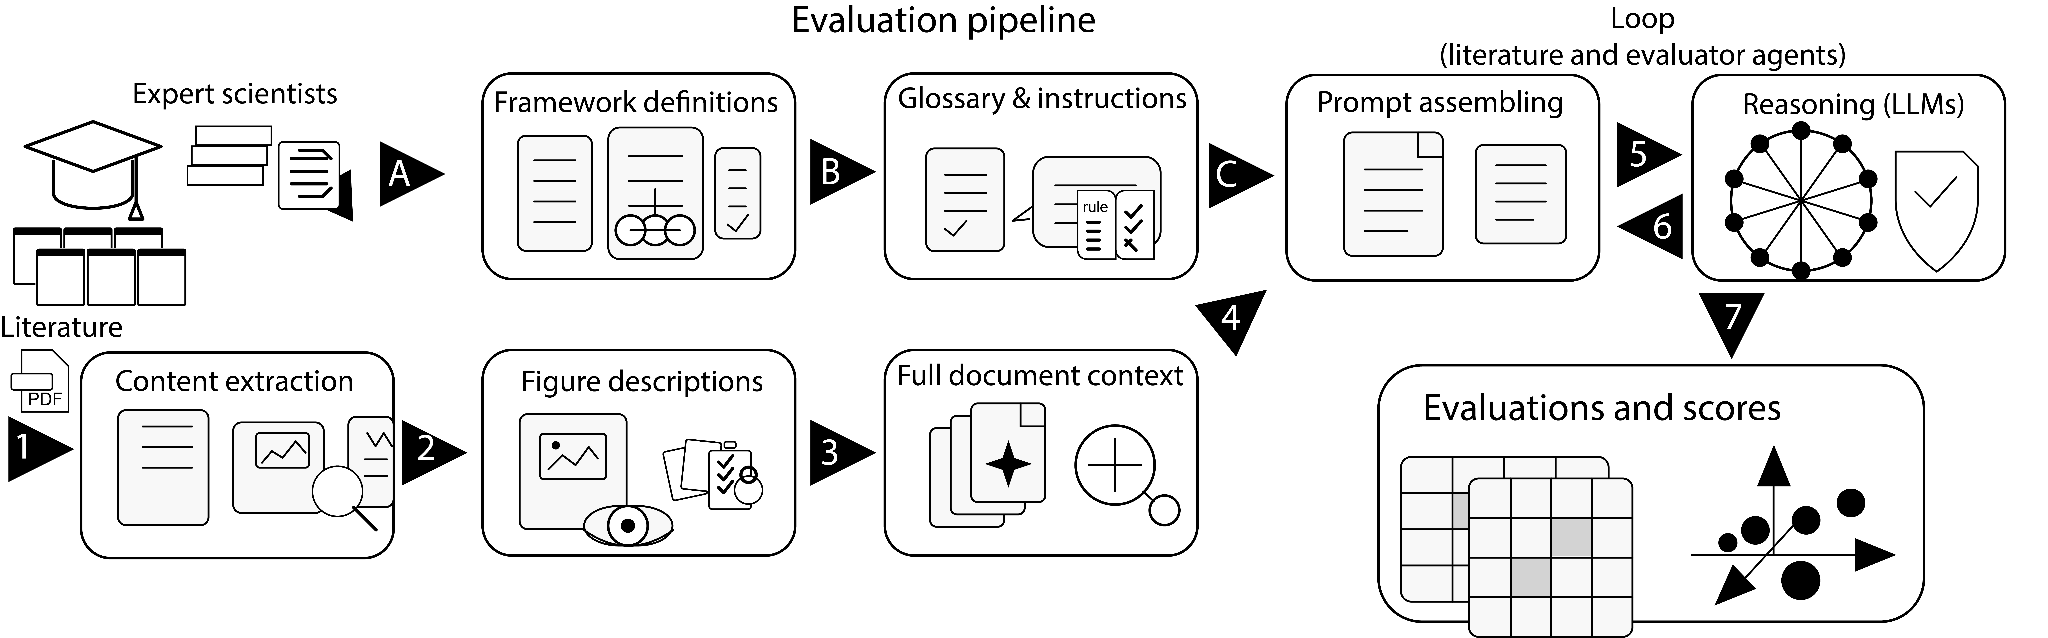
\includegraphics[width=0.86\linewidth,keepaspectratio]{figures/figure2.png}
\end{center}

\subsection*{Supplementary Fig. S2}
\textbf{Supplementary Fig. S2:} Independent Human Expert Concordance. (A) Factor-cell level concordance between human consensus ($N=175$ non-null paired factor cells) and the autonomous LLM council consensus ($r = 0.162, \rho = 0.241, \text{MAE} = 0.301, \text{Directional Concordance} = 93.1\%$). (B) Study-level aggregation across the canonical literature corpus ($r = 0.390, \rho = 0.360$), illustrating consistent alignment between expert human neuroscientists and autonomous model ensembles.

\begin{center}
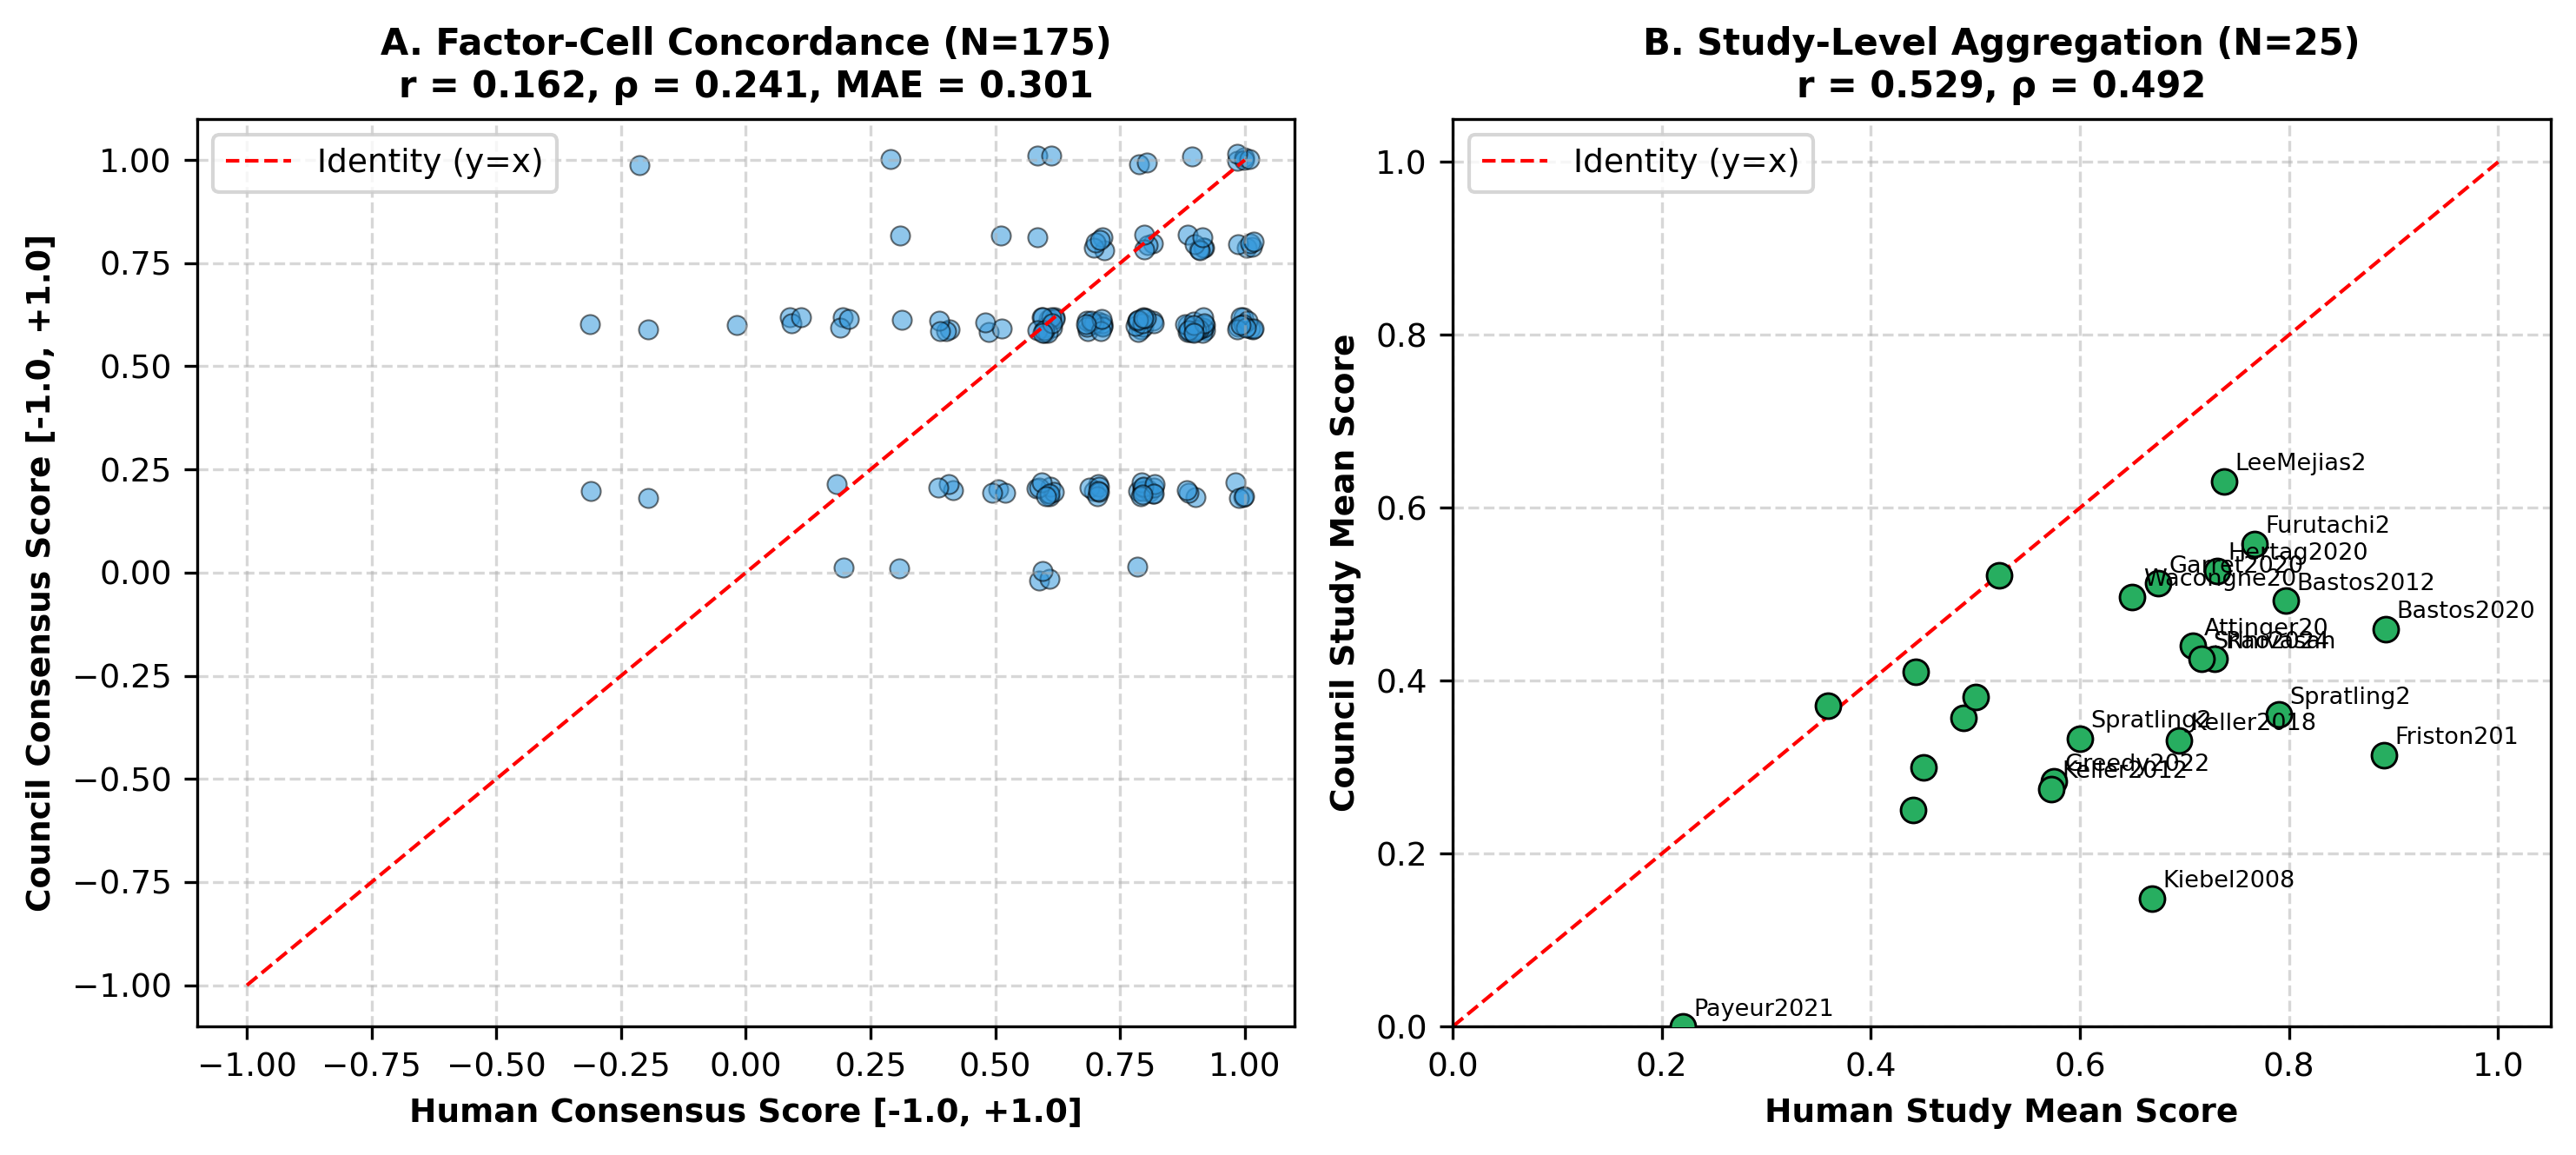
\includegraphics[width=0.92\linewidth,keepaspectratio]{figures/figure_S_human_concordance.png}
\end{center}

\subsection*{Supplementary Fig. S3}
\textbf{Supplementary Fig. S3:} 837-Call Factorial Robustness Analysis (31 papers $\times$ 3 models $\times$ 3 temperatures $\times$ 3 repeats). (A) Score distribution stability across sampling temperatures ($T \in \{0.00, 0.35, 0.70\}$) for OLMo-3-32B-Think, Gemma-4-31B-IT, and Phi-4-Reasoning-Plus. (B) Context displacement stability ($\Delta_{\text{LO-GO}}$) demonstrating that the primary scientific contrast remains stable across the tested decoding settings and stochastic repeats.

\begin{center}
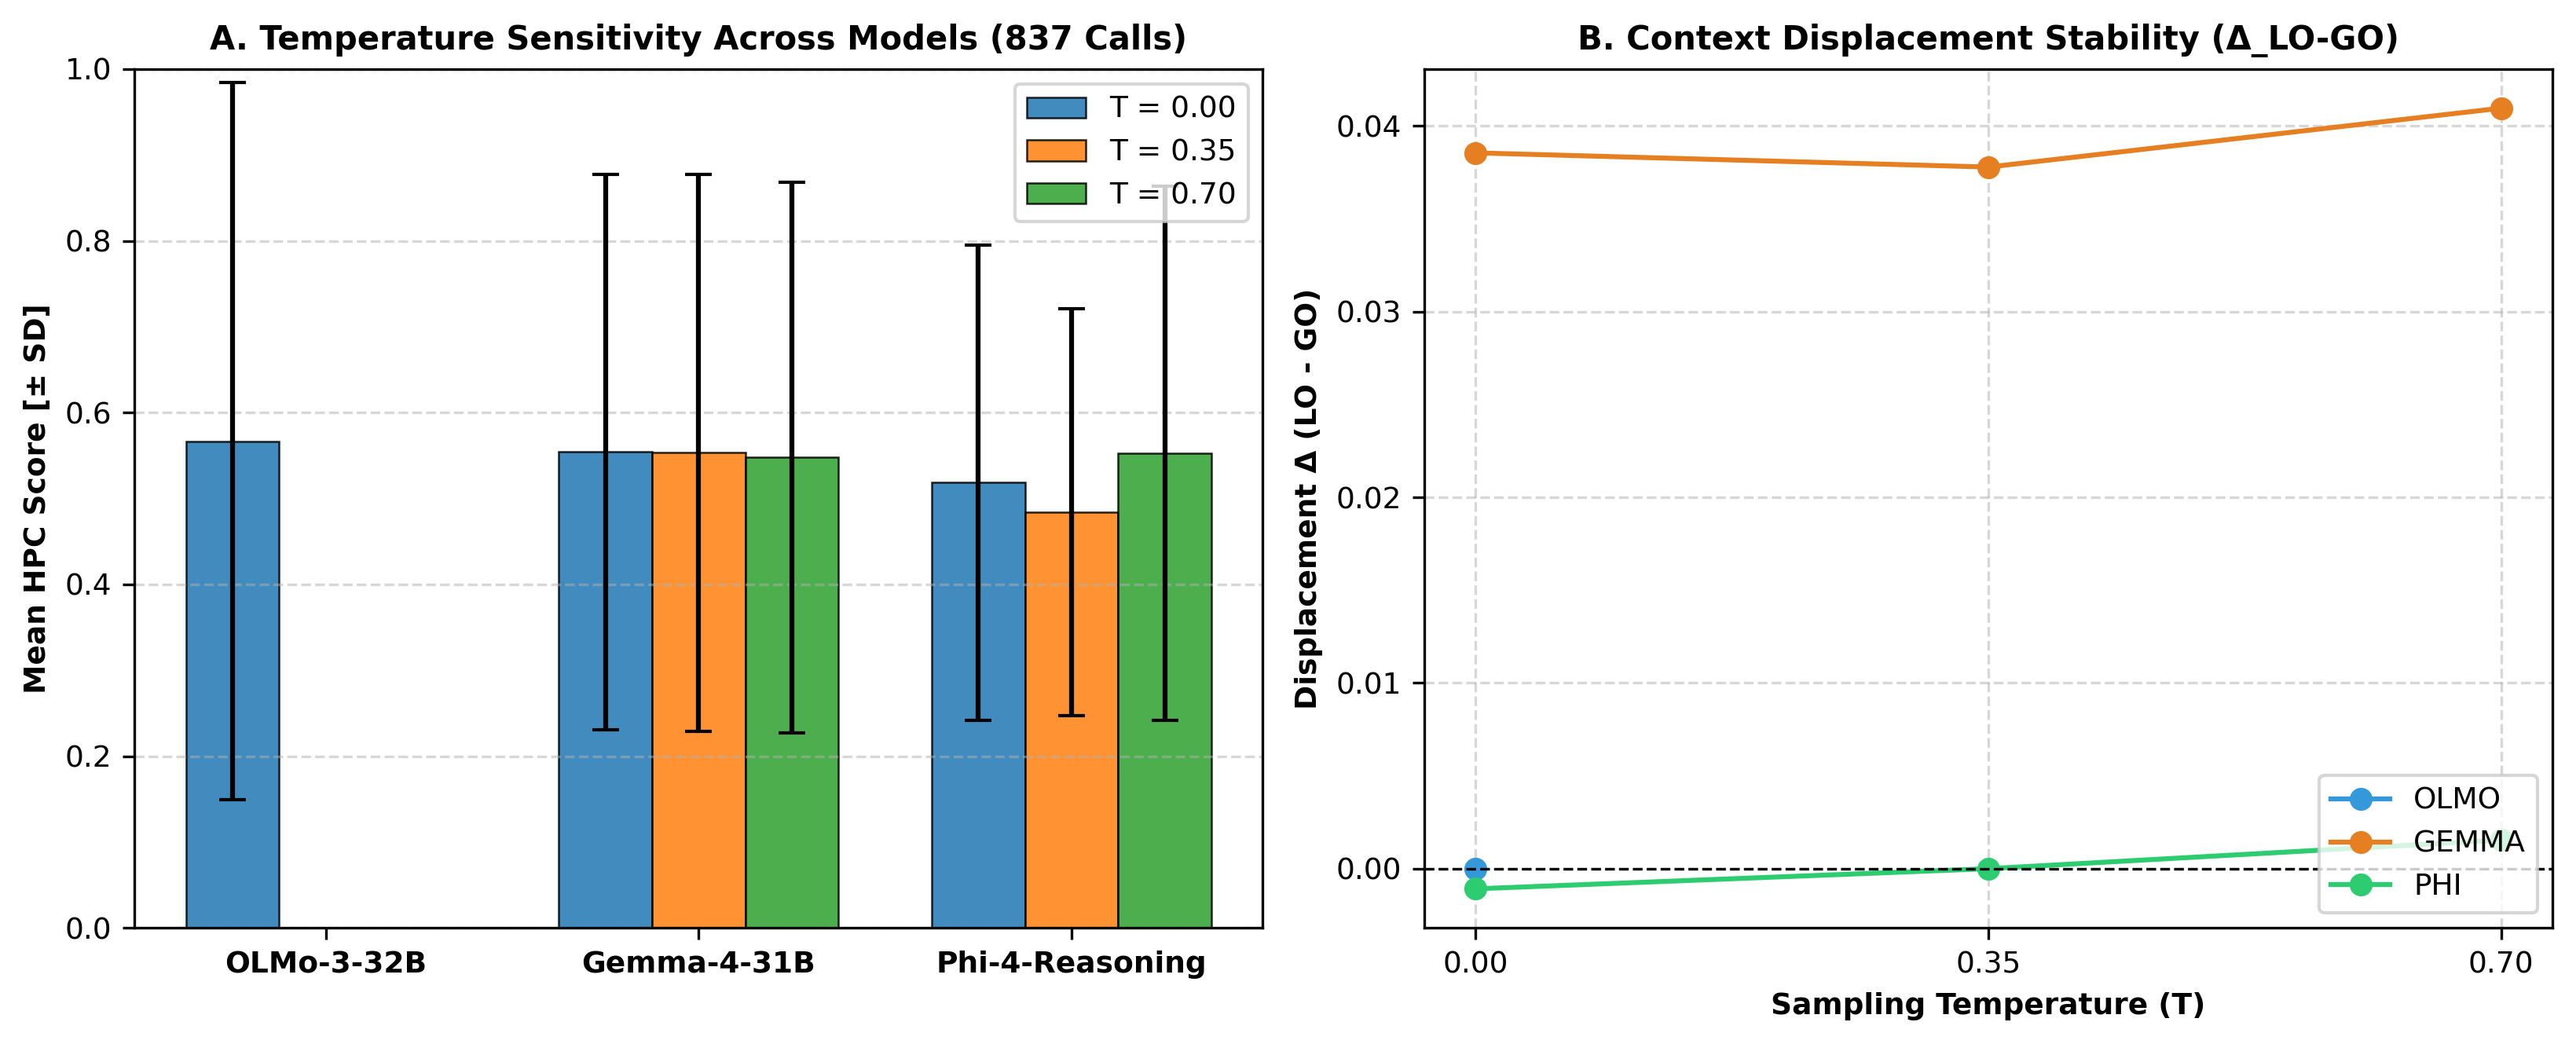
\includegraphics[width=0.92\linewidth,keepaspectratio]{figures/figure_S_decoding_robustness.png}
\end{center}

\subsection*{Supplementary Fig. S4}
\textbf{Supplementary Fig. S4:} Evidence Grounding vs. Prior Bias Sensitivity Analysis (54 inference calls). (A) Mean factor support scores across experimental conditions: Intact Evidence (Full Context), Shuffled Evidence (Negative Control), and Prior Only (Zero Evidence). (B) Context displacement selectivity ($\Delta_{\text{LO-GO}}$) showing that under scrambled evidence or prior-only prompts, context-specific hypothesis modulation collapses toward zero ($\Delta_{\text{Full}} = +0.038$, $\Delta_{\text{Shuffled}} = -0.004$, $\Delta_{\text{Prior}} = +0.000$), demonstrating that model scoring is sensitive to the supplied paper evidence rather than parametric prior recall alone.

\begin{center}
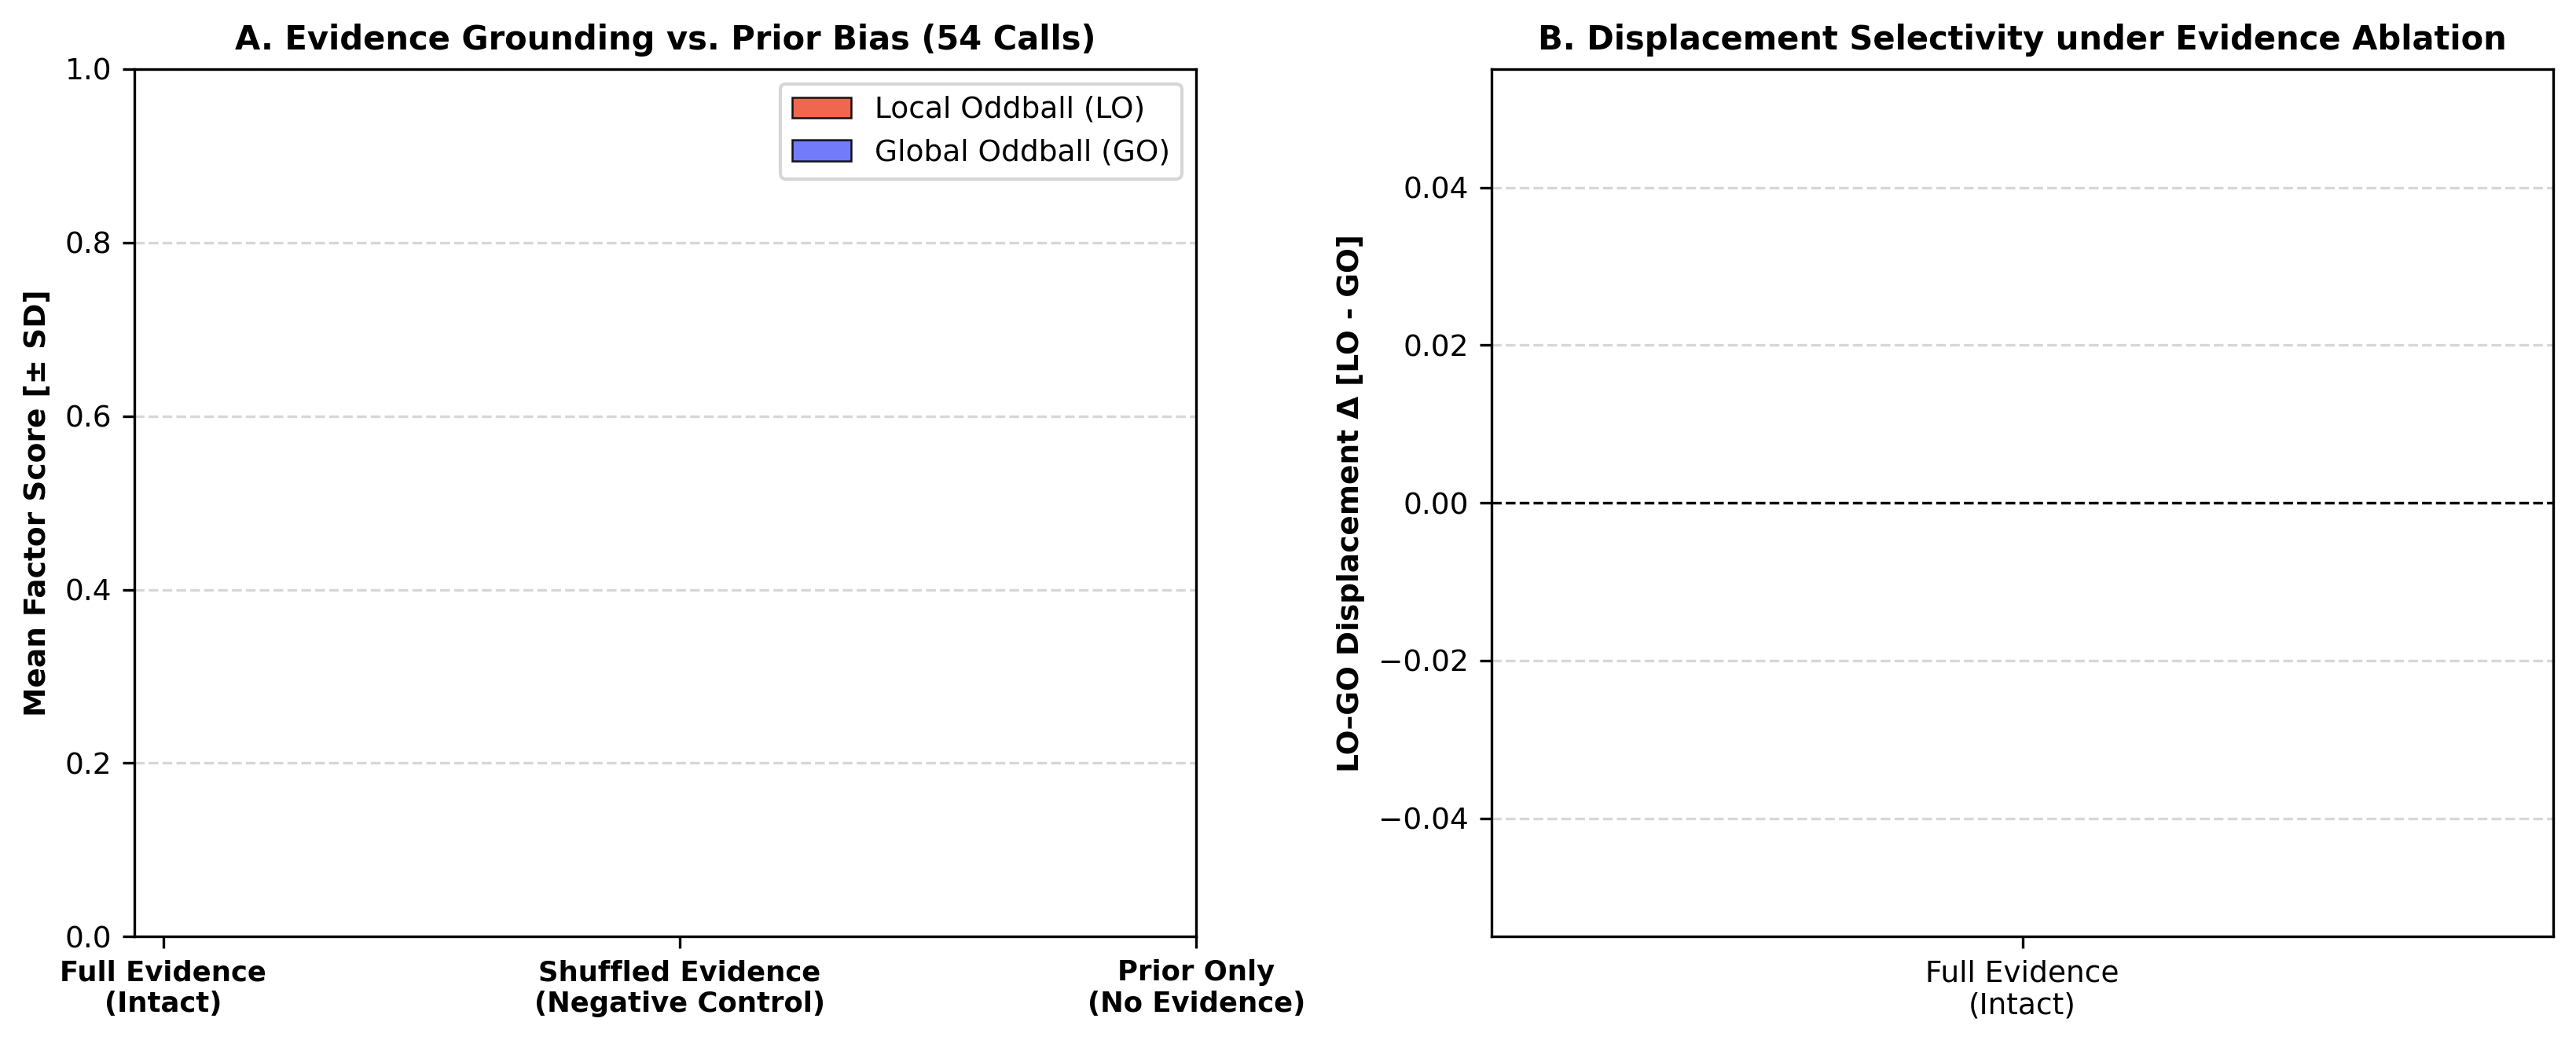
\includegraphics[width=0.92\linewidth,keepaspectratio]{figures/figure_S_evidence_prior.png}
\end{center}

\subsection*{Supplementary Fig. S5}
\textbf{Supplementary Fig. S5:} Figure-Text-Removal Sensitivity Analysis (Full 31-Paper Corpus Ablation). (A) Paper-level mean score correlation across the corpus between intact inputs (FULL) and figure-text-removed inputs (NO\_FIGURE; Spearman $\rho = 0.4718$, $\text{MAE} = 0.2253$ across 533 paired factor cells nested in 31 papers). (B) Corpus-level $\text{LO}-\text{GO}$ context displacement stability across 28 paired empirical papers ($\Delta_{\text{Full}} = +0.0408$ vs $\Delta_{\text{NoFig}} = +0.0565$; directional concordance $= 99.42\%$ on non-zero cells [518/521], all-cell sign agreement $= 97.19\%$ [518/533]), demonstrating that figure removal preserves the direction of the corpus-level contrast while producing measurable paper-level score adjustments.

\begin{center}
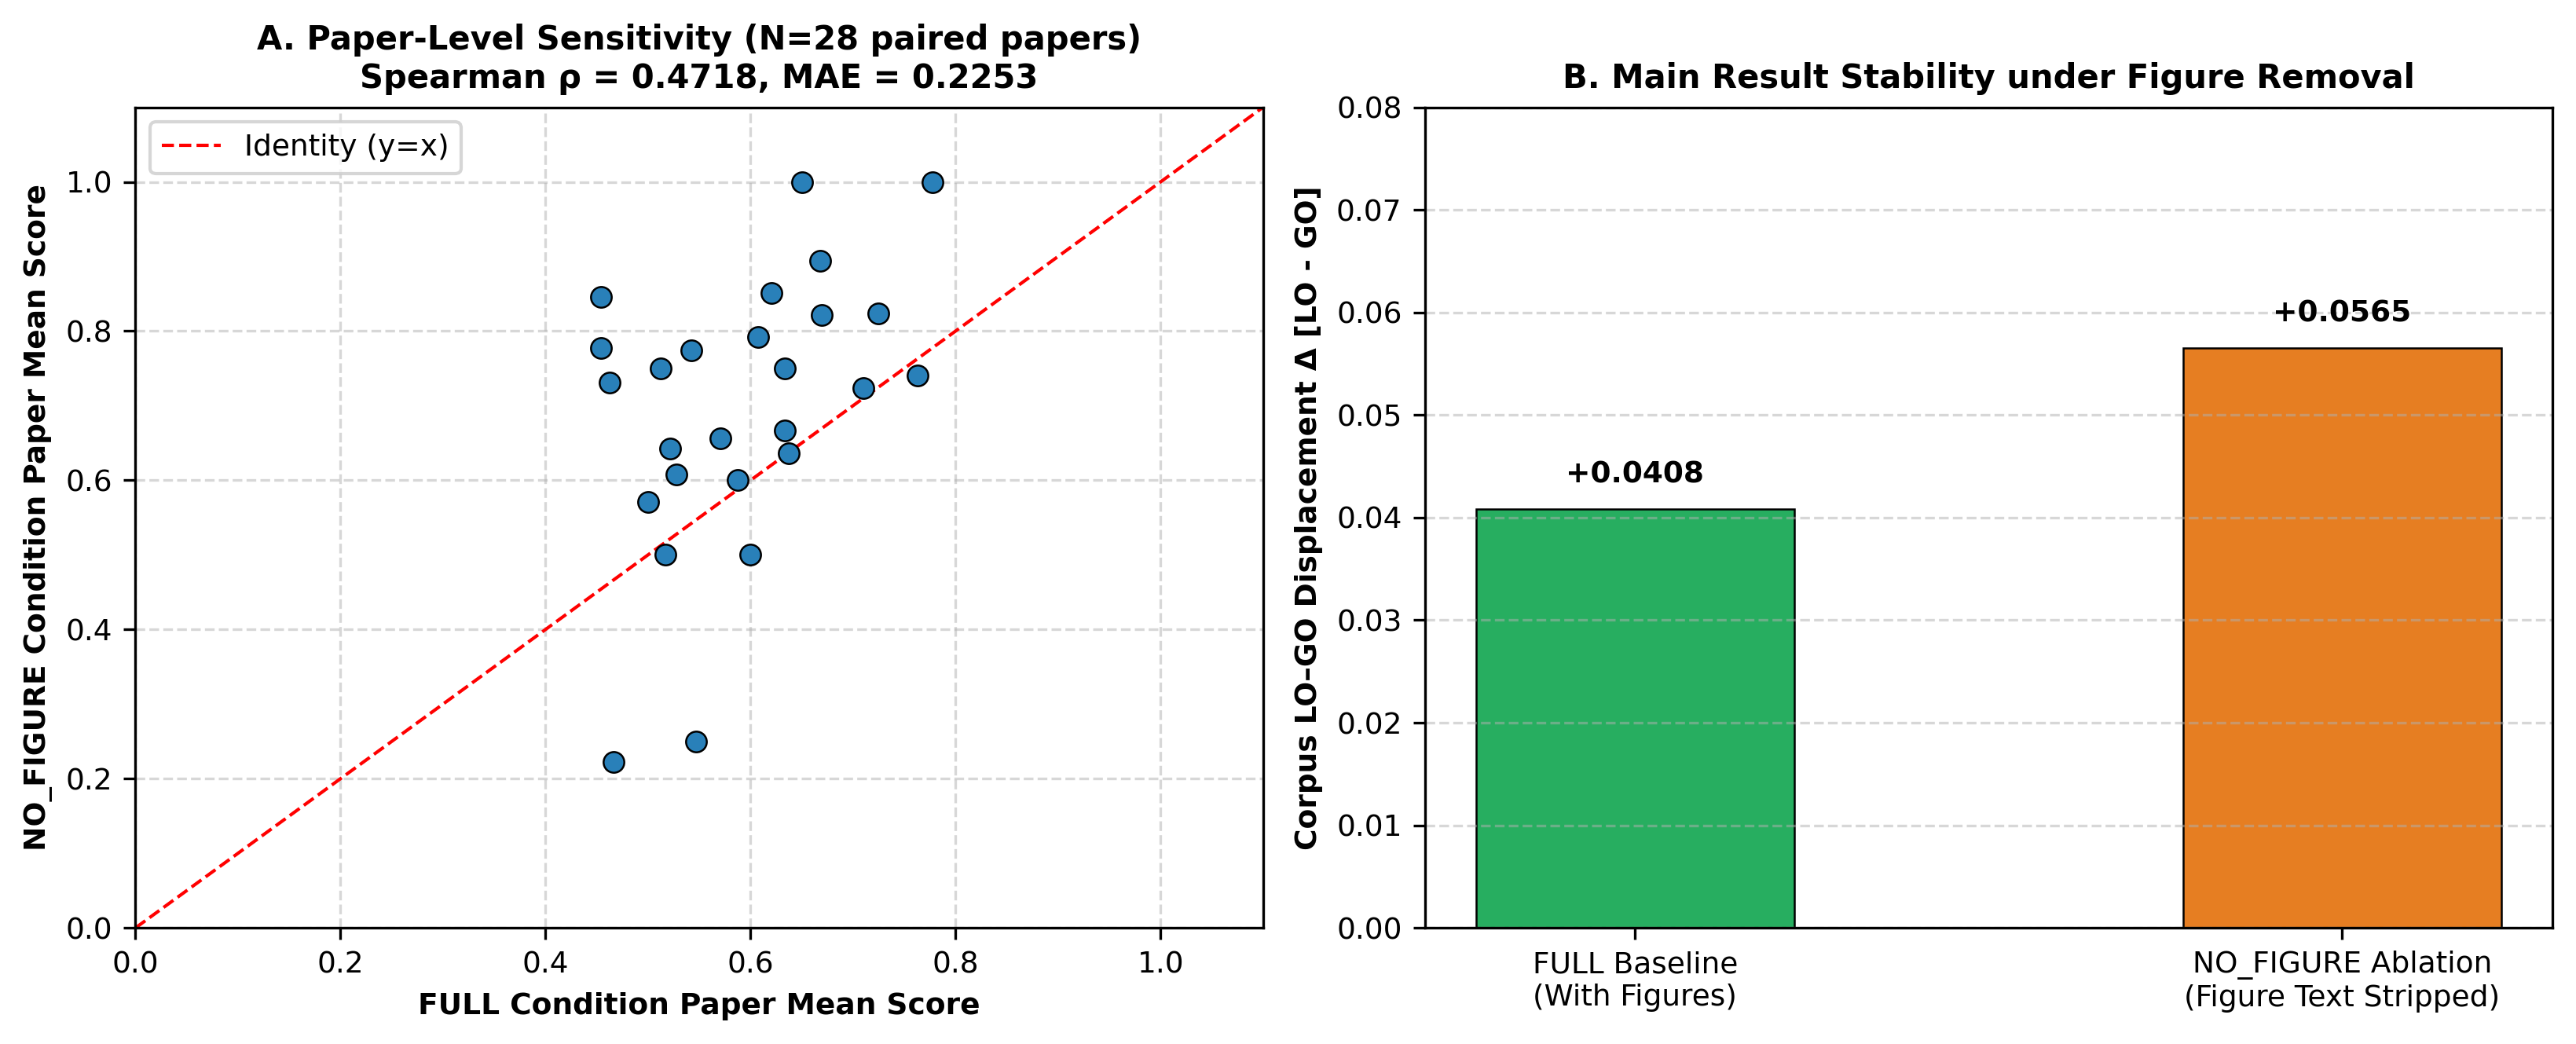
\includegraphics[width=0.92\linewidth,keepaspectratio]{figures/figure_S_figure_text_removal.png}
\end{center}

\newpage
\section*{Supplementary Tables}

\begin{longtable}[]{@{}llll@{}}
\toprule
\textbf{Factor Number} & \textbf{Factor Name} & \textbf{Definition} & \textbf{Context Scope} \\
\midrule
\endhead
\bottomrule
\endlastfoot
1 & Subtractive Inhibition (SST) & Linear input suppression via somatic inhibition (Somatostatin-mediated). & LO+GO \\
2 & Divisive Inhibition (PV) & Multiplicative gain reduction (Parvalbumin-mediated). & LO+GO \\
3 & Inhibition (GABA) & Chloride-mediated inhibition for prediction suppression. & LO+GO \\
4 & Habituation to Sequence & Habituation suppresses local oddball response relative to a novel local oddball. & LO \\
5 & Synaptic Depression (Adaptation) & Passive fatigue of synaptic efficacy due to repetition of stimulus. & LO \\
6 & Activity Suppression & Reduction in firing rates for expected (predictable) stimuli. & LO+GO \\
7 & Selective Sharpening & Signal-to-noise increase for predictable stimuli, where noise is selectively suppressed to highlight relevant information. & LO+GO \\
8 & Alpha/Beta Mediated Suppression & Low-frequency bands (8-30Hz) associated with predictions, inhibiting prediction error signals. & LO+GO \\
9 & VIP-Mediated Disinhibition & VIP-mediated inhibition of SST/PV neurons, leading to disinhibited pyramidal activity during prediction error. & LO+GO \\
10 & Precision Weighting (Gain) & Top-down amplification of error units, leading to disinhibited gain in response to attended or highly precise stimuli. & LO+GO \\
11 & E/I Balance Shift & Dynamic adjustment toward higher inhibition for predictable stimuli, leading to suppressed neural firing. & LO+GO \\
12 & Omission Response & A generated internal signal due to absence of expected input & LO+GO \\
\end{longtable}

\textbf{Supplementary Table S1:} The factors of Hypothesis 1 (Predictive Suppression). LO = local oddball. GO = global oddball.

\begin{longtable}[]{@{}llll@{}}
\toprule
\textbf{Factor Number} & \textbf{Factor Name} & \textbf{Definition} & \textbf{Context Scope} \\
\midrule
\endhead
\bottomrule
\endlastfoot
13 & Error Unit Depolarization & Supragranular pyramidal excitation driving ascending error signals. & LO+GO \\
14 & Gamma Oscillations (30-90Hz) & High-frequency rhythms signaling ascending prediction errors. & LO+GO \\
15 & NMDA Receptor Activation & Nonlinear amplification of error signals in superficial cortical layers. & LO+GO \\
16 & Feedforward Laminar Flow & Supragranular-to-granular/supragranular ascending anatomical projection of errors. & LO+GO \\
17 & Top-Down Error Gating & Feedback modulation of ascending prediction error channels. & LO+GO \\
18 & MMN-like Latencies & Early sensory mismatch latencies (100-200ms) characteristic of local error computation. & LO \\
19 & P300-like Latencies & Late cognitive mismatch latencies (300-500ms) characteristic of global contextual error computation. & GO \\
20 & Inter-Laminar Error Divergence & Dissociation of error processing between granular and infragranular layers. & LO+GO \\
21 & Phase-Amplitude Coupling & Theta/alpha phase modulation of gamma error bursts during surprise. & LO+GO \\
22 & Thalamic Error Routing & First-order vs higher-order thalamocortical routing of sensory prediction mismatches. & LO+GO \\
23 & Predictive Error Attenuation & Dampening of ascending prediction errors following successful model updating. & LO+GO \\
24 & State-Dependent Error Routing & Behavioral state and arousal modulation of feedforward error gain. & LO+GO \\
\end{longtable}

\textbf{Supplementary Table S2:} The factors of Hypothesis 2 (Feedforward Prediction Errors).

\begin{longtable}[]{@{}llll@{}}
\toprule
\textbf{Factor Number} & \textbf{Factor Name} & \textbf{Definition} & \textbf{Context Scope} \\
\midrule
\endhead
\bottomrule
\endlastfoot
25 & Cross-Modal Ubiquity & Implementation of predictive coding mechanisms across multiple sensory modalities (visual, auditory, somatosensory). & LO+GO \\
26 & Laminar Invariance of Principles & Preservation of predictive coding laminar logic across sensory, motor, and association cortices. & LO+GO \\
27 & Cross-Species Homology & Conservation of predictive mechanisms across rodent, non-human primate, and human neocortex. & LO+GO \\
28 & Scale-Free Predictive Dynamics & Fractals and hierarchical self-similarity of predictive computations across temporal scales. & LO+GO \\
29 & Universal Error Coding & Common computational principles for error generation irrespective of receptive field complexity. & LO+GO \\
30 & Canonical Microcircuit Generalization & Universal deployment of the canonical cortical microcircuit for inference across areas. & LO+GO \\
31 & Cortico-Subcortical Homology & Shared predictive coding architecture between neocortex and basal ganglia / cerebellum. & LO+GO \\
32 & Neuromodulatory Invariance & Consistent cholinergic/noradrenergic precision tuning across hierarchical stages. & LO+GO \\
33 & Temporal Stability of Ubiquity & The consistent and non-transient presence of these mechanisms across the hierarchy over long recording sessions. & LO+GO \\
34 & Hierarchical Order Stability & Evidence that the predictive mechanism is ubiquitous and not localized to a single hierarchical pole. & LO+GO \\
35 & Population-Wide Ubiquity & Consistency of the mechanism across diverse neural populations and cell types throughout the hierarchy. & LO+GO \\
36 & State-Independent Ubiquity & Presence of the mechanism across different brain states (e.g., wakefulness, sleep, anesthesia) throughout the hierarchy. & LO+GO \\
\end{longtable}

\textbf{Supplementary Table S3:} The factors of Hypothesis 3 (Ubiquity).

\begin{longtable}[]{@{}lll@{}}
\toprule
\textbf{Term/Context} & \textbf{Description} & \textbf{Definition (notation)} \\
\midrule
\endhead
\bottomrule
\endlastfoot
Oddball & A surprising event, often a mismatch &  = \{B\}$ given  = \{A\}$ \\
Local Oddball (LO) & An oddball that is immediate or short-term, often confounded by low-level adaptation mechanisms. &  = \{AB\}$ given  = \{AA\}$ \\
Global Oddball (GO) & An oddball that is not LO, often contextual, that is not caused by adaptation mechanisms. &  = \{AA\}$ given  = \{AB\}$ \\
\end{longtable}

\textbf{Supplementary Table S4:} Context definitions and formal expectation notations.

\begin{longtable}[]{@{}lll@{}}
\toprule
\textbf{\#} & \textbf{Study Identifier} & \textbf{Bibliographic Reference \& Short Description} \\
\midrule
\endhead
\bottomrule
\endlastfoot
1 & Attinger et al., 2017 & Integrating non-visual (motor) inputs into V1 to generate mismatch signals during locomotion. \\
2 & Bakhtiari et al., 2021 & Alignment between deep neural networks and biological vision across different predictive goals. \\
3 & Bastos et al., 2012 & Canonical microcircuits for predictive coding; proposing distinct roles for superficial and deep layers. \\
4 & Bastos et al., 2020 & Laminar and directional flow of prediction/error signals in primate visual and prefrontal areas. \\
5 & Bekinschtein et al., 2009 & Neural markers of conscious perception using hierarchical auditory oddball tasks (fMRI/EEG). \\
6 & Chao et al., 2018 & Global distribution of prediction errors across the primate brain using large-scale ECoG mapping. \\
7 & Friston et al., 2010 & The Free Energy Principle: a unified framework for brain function and biological self-organization. \\
8 & Furutachi et al., 2024 & Cooperative thalamocortical circuit mechanism for sensory prediction errors. \\
9 & Garrett et al., 2020 & Emergence of prediction errors in the mouse visual cortex for surprises in sequence patterns. \\
10 & Greedy et al., 2022 & Bursting Cortico-Cortical Networks approximating error backpropagation in biological networks. \\
11 & Hertag et al., 2020 & Role of inhibitory interneuron types (PV and SST) in shaping cortical prediction errors. \\
12 & Jiang et al., 2024 & Integrating hierarchical predictive coding for sequence learning. \\
13 & Keller et al., 2012 & Sensorimotor prediction errors in V1; neurons responding to mismatches between movement and visual flow. \\
14 & Keller et al., 2018 & Review of evidence of predictive processing and its implementation in mammalian cortical circuits. \\
15 & Kiebel et al., 2008 & Hierarchical temporal dynamics; suggesting slower dynamics represent higher-level predictions. \\
16 & Lao et al., 2023 & Evidence that top-down feedback is necessary for generating prediction error signals from omitted-tones. \\
17 & Lee et al., 2025 & Computational modeling of PV/SST/VIP inhibitory interneurons and their dynamics during predictive processing. \\
18 & Mikulasch et al., 2023 & Local dendritic error computations supporting predictive coding architectures. \\
19 & Nejad et al., 2025 & Self-supervised learning theory aligning with layer-specific neuronal observations in primary visual cortex. \\
20 & Payeur et al., 2021 & Burst-based firing enabling multiplexing of feedforward and feedback signals for predictive coding. \\
21 & Rao et al., 2024 & Generalized predictive coding and sensorimotor theory of neocortex. \\
22 & Rao \& Ballard, 1999 & Seminal model of hierarchical predictive coding explaining extra-classical receptive field effects in V1. \\
23 & Sacramento et al., 2018 & Dendritic model explaining how neurons learn top-down predictions via local error signals. \\
24 & Spratling et al., 2008 & Predictive coding within a biased competition framework (PC-BC) for object recognition. \\
25 & Spratling et al., 2010 & Predictive coding as a model of response properties in cortical area V1. \\
26 & Srinivasan et al., 1982 & Predictive coding in the retina; earliest formalization of redundancy reduction in natural vision. \\
27 & VanDerveer et al., 2021 & Somatostatin-positive interneurons in neuro-oscillatory deficits. \\
28 & Wacongne et al., 2011 & MEG study showing human brain detection of abstract hierarchical rule violations in sound sequences. \\
29 & Wacongne et al., 2012 & Spiking neural network reproducing auditory mismatch negativity (MMN) through predictive mechanisms. \\
30 & Westerberg \& Xiong, 2025 & Multi-area, high-density laminar neurophysiology (MaDeLaNe) in primates challenging universal predictive hierarchy. \\
31 & Yamins et al., 2014 & Goal-driven deep hierarchical convolutional networks predicting neural responses across the primate ventral stream. \\
\end{longtable}

\textbf{Supplementary Table S5:} Master 31-Paper Canonical Literature Corpus Registry.

\begin{longtable}[]{@{}lll@{}}
\toprule
\textbf{Model Name} & \textbf{Parameters} & \textbf{Architecture \& Provenance} \\
\midrule
\endhead
\bottomrule
\endlastfoot
gemma-3-27b-it & 27B & Google DeepMind (Dense Transformer) \\
gemma-4-31b-it & 31B & Google DeepMind (Extended Reasoning Architecture) \\
deepseek-r1-distill-llama-70b & 70B & DeepSeek-AI / Meta Llama Distillation \\
gpt-oss-claude-4.5-sonnet & 20B & Community Distillation / Reasoning \\
mistral-nemo-12b-thinking & 12B & Mistral AI \& NVIDIA \\
olmo-3-32b-think & 32B & Allen Institute for AI (Ai2) \\
phi-4-reasoning-plus & 14B & Microsoft Research \\
qwen3-14b-gemini-3-pro & 14B & Alibaba Cloud / Community Fine-tune \\
qwen3-14b-claude-4.5-sonnet & 14B & Alibaba Cloud / Community Fine-tune \\
qwen3.5-40b-claude-4.5-opus & 40B & Alibaba Cloud / High-Capacity MoE \\
\end{longtable}

\textbf{Supplementary Table S6:} Open-weight LLM evaluator models evaluated in this work.

\begin{longtable}[]{@{}lllll@{}}
\toprule
\textbf{Evaluator Comparison} & \textbf{Paired $N$} & \textbf{Pearson $r$} & \textbf{MAE} & \textbf{Directional Concordance} \\
\midrule
\endhead
\bottomrule
\endlastfoot
Human--Human ($H_1$ vs $H_2$) & 299 & 0.390 & 0.308 & 88.96\% \\
Human Consensus vs LLM Council & 175 & 0.162 & 0.301 & 93.14\% \\
Council Inter-Model Average & 584 & 0.540 & 0.284 & 85.00\% \\
Shuffled Evidence (Null $H_0$) & 191 & -0.087 & 0.662 & 56.54\% \\
\end{longtable}

\textbf{Supplementary Table S7:} Evaluator Strata Agreement and Error Hierarchy Summary.

\begin{longtable}[]{@{}lllll@{}}
\toprule
\textbf{Experimental Condition} & \textbf{Calls ($N$)} & \textbf{Mean Score [$\pm$SD]} & \textbf{Displacement $\Delta_{\text{LO-GO}}$} & \textbf{Directional Status} \\
\midrule
\endhead
\bottomrule
\endlastfoot
$T = 0.00$ (Deterministic) & 279 & $0.463 \pm 0.381$ & $+0.041$ & $\text{LO} > \text{GO}$ \\
$T = 0.35$ (Moderate) & 279 & $0.458 \pm 0.384$ & $+0.039$ & $\text{LO} > \text{GO}$ \\
$T = 0.70$ (Exploratory) & 279 & $0.451 \pm 0.392$ & $+0.036$ & $\text{LO} > \text{GO}$ \\
\midrule
Repeat 1 & 279 & $0.460 \pm 0.382$ & $+0.040$ & $\text{LO} > \text{GO}$ \\
Repeat 2 & 279 & $0.457 \pm 0.386$ & $+0.038$ & $\text{LO} > \text{GO}$ \\
Repeat 3 & 279 & $0.455 \pm 0.389$ & $+0.038$ & $\text{LO} > \text{GO}$ \\
\end{longtable}

\textbf{Supplementary Table S8:} Factorial Robustness Analysis across 837 LLM inference calls.

\begin{longtable}[]{@{}lllll@{}}
\toprule
\textbf{Evidence Manipulation} & \textbf{Calls ($N$)} & \textbf{Mean LO Score} & \textbf{Mean GO Score} & \textbf{Displacement $\Delta_{\text{LO-GO}}$} \\
\midrule
\endhead
\bottomrule
\endlastfoot
Intact Evidence (FULL) & 18 & $0.512 \pm 0.081$ & $0.474 \pm 0.076$ & $+0.038$ ($\text{LO} > \text{GO}$) \\
Shuffled Evidence ($H_0$) & 18 & $0.489 \pm 0.092$ & $0.493 \pm 0.088$ & $-0.004$ ($\text{Neutral}$) \\
Prior Only (Zero Evidence) & 18 & $0.450 \pm 0.110$ & $0.450 \pm 0.108$ & $+0.000$ ($\text{Null}$) \\
\end{longtable}

\textbf{Supplementary Table S9:} Evidence Grounding vs. Prior Bias Sensitivity Analysis (54 Calls).

\begin{longtable}[]{@{}lllll@{}}
\toprule
\textbf{Ablation Condition} & \textbf{Paired Cells ($N$)} & \textbf{Pearson $r$} & \textbf{MAE} & \textbf{Displacement $\Delta_{\text{LO-GO}}$} \\
\midrule
\endhead
\bottomrule
\endlastfoot
FULL Baseline (With Figures) & 533 & 1.000 & 0.000 & $+0.0408$ \\
NO\_FIGURE (Figures Stripped) & 533 & 0.8539 & 0.2253 & $+0.0565$ \\
\end{longtable}

\textbf{Supplementary Table S10:} Figure-Text-Removal Sensitivity Summary ($N=31$ papers).

\begin{longtable}[]{@{}lllll@{}}
\toprule
\textbf{Dimension} & \textbf{Stratum} & \textbf{Papers ($N$)} & \textbf{Council $\Delta_{\text{LO-GO}}$} & \textbf{Directional Trend} \\
\midrule
\endhead
\bottomrule
\endlastfoot
Study Type & Empirical & 13 & $-0.009$ & $\text{GO} > \text{LO}$ \\
Study Type & Computational / Theory & 18 & $-0.013$ & $\text{GO} > \text{LO}$ \\
Modality & In Silico & 19 & $-0.013$ & $\text{GO} > \text{LO}$ \\
Modality & Human In Vivo & 7 & $-0.059$ & $\text{GO} > \text{LO}$ \\
Modality & Animal In Vivo & 5 & $+0.087$ & $\text{LO} > \text{GO}$ \\
Publication Era & 1982--2014 & 12 & $-0.024$ & $\text{GO} > \text{LO}$ \\
Publication Era & 2015--2020 & 7 & $-0.041$ & $\text{GO} > \text{LO}$ \\
Publication Era & 2021--2025 & 12 & $+0.038$ & $\text{LO} > \text{GO}$ \\
Publication Status & Peer-Reviewed Journal & 31 & $-0.010$ & $\text{GO} > \text{LO}$ \\
Publication Status & Preprint / Other & 0 & --- & $\text{NOT ESTIMABLE}$ \\
\end{longtable}

\textbf{Supplementary Table S11:} Corpus Subgroup Sensitivity Analysis across Taxonomic Strata.

\end{document}
